\documentclass[8pt,pdf,hyperref={unicode}]{beamer}

% \documentclass[aspectratio=43]{beamer}
% \documentclass[aspectratio=1610]{beamer}
% \documentclass[aspectratio=169]{beamer}

\usepackage{lmodern}
\usepackage[russian]{babel}
\usepackage{subcaption}

% подключаем кириллицу 
\usepackage[T2A]{fontenc}
\usepackage[utf8]{inputenc}

\usepackage{mathrsfs} % буква для обозначения ЭДС
\newcommand{\EDS}{\ensuremath{\mathscr{E}}} % новая команда \EDS для символа

% отключить клавиши навигации
\setbeamertemplate{navigation symbols}{}

% тема оформления
\usetheme{CambridgeUS}

% цветовая схема
\usecolortheme{Beaver}

\title{Тепловые свойства твердых тел}   
\subtitle{Лабораторная работа}
\author{Никитин Илья} 
\date{\today}

\begin{document}
	
	\maketitle
	
\begin{frame}
	\frametitle{План доклада}
	\begin{center}
		\begin{itemize}
			\item Теоретическое введение
			\item Оборудование
			\item Измерение температурных коэффициентов
			\item Определение мощности и теоретических коэффициентов
		\end{itemize}
	\end{center}
\end{frame}
\begin{frame}
	\frametitle{Теория}
	\framesubtitle{Зависимость удельного сопротивления от температуры}
	\begin{center}
		Зависимость удельного сопротивления от температуры:
		\begin{equation}
		\rho = \rho_0 [1 + \alpha(T - T_0)]
		\end{equation}
		Закон Ньютона-Рихмана:
		\begin{equation}
		q_n = \beta (T - T_0)
		\end{equation}
	\end{center}
\end{frame}
\begin{frame}
	\frametitle{Теория}
	\framesubtitle{Тепловое излучение}
	\begin{center}
	Согласно закону Стефана-Больцмана:
\begin{equation}
dP = \epsilon \sigma (T^4 - T^4_0)dS
\end{equation}
где $\sigma = \frac{2 \pi^5 k^4_B}{15h^3c^2}$	
	\end{center}
\end{frame}
\begin{frame}
	\frametitle{Теория}
	\framesubtitle{Тепловое излучение}
	\begin{center}
	В стационарном режиме вся установившаяся мощность $P_{st} = I^2 R_{st}$ равна суммарной мощности тепловых потерь:
	\begin{equation}
	P_{st} = \beta S_{surf} (T - T_0) + \epsilon \sigma S_{surf} (T^4 - T^4_0)
	\end{equation}			
	\end{center}
\end{frame}
\begin{frame}
	\frametitle{Оборудование}
	\begin{center}
		\begin{itemize}
			\item Проволоки из различных материалов
			\item Термопаста КПТ-19
			\item Алюминевая банка
			\item Термопара К-типа
			\item Мультиметр
			\item Шунт
			\item Два мультиметра Keysight
			\item Коробка картонная
			\item Клемник
			\item Компьютер с программой LabView
			\item Электрический кипятильник
			\item Источник тока Gophert
			\item Резинки для зажима проволоки
		\end{itemize}
	\end{center}
\end{frame}
\begin{frame}
	\frametitle{Ход работы}
	\framesubtitle{Измерение температурных коэффициентов}
	\begin{center}
		\begin{figure}[h!]
			\centering
			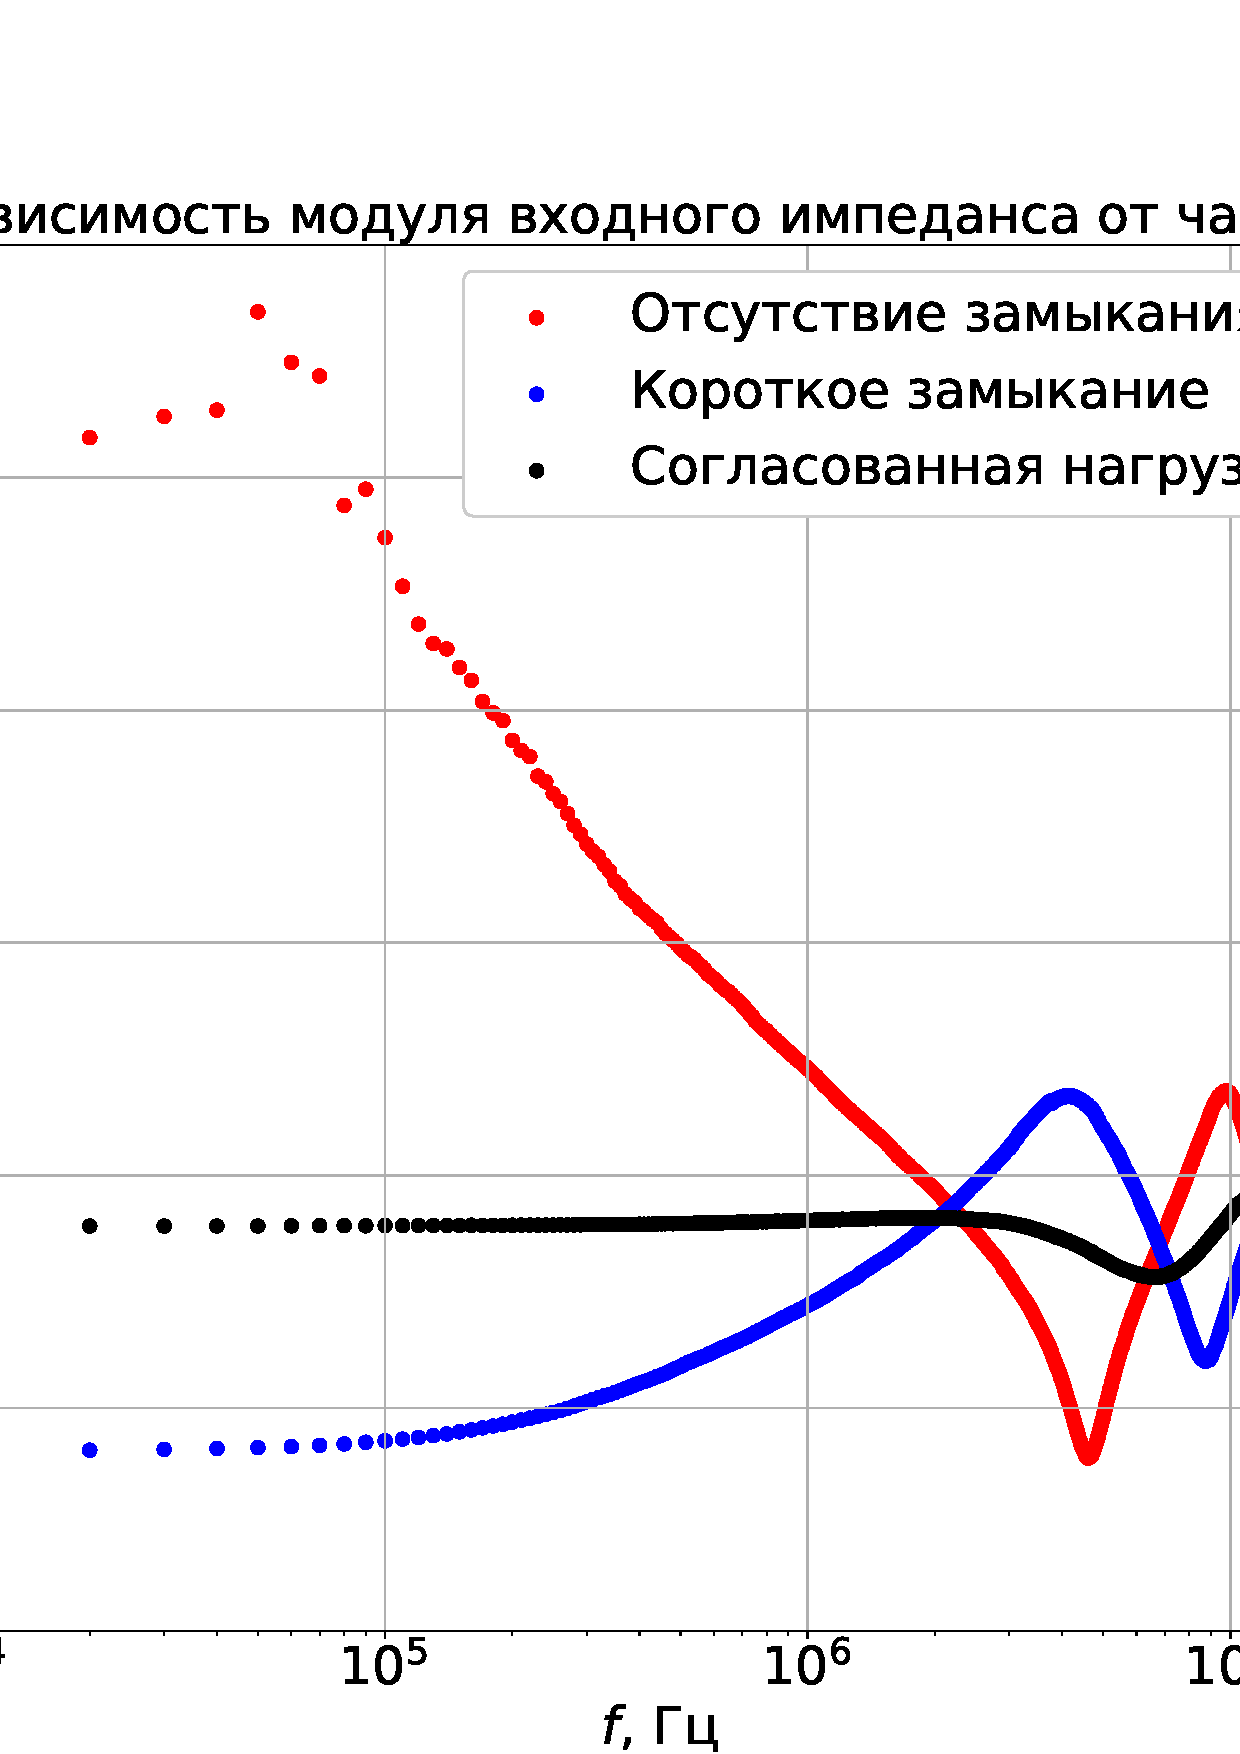
\includegraphics[width=.6\linewidth]{Lab3_1.png}
			\caption{Схема подключения проволоки}
			\label{fig1}
		\end{figure}		
	\end{center}
\end{frame}
\begin{frame}
	\frametitle{Ход работы}
	\framesubtitle{Измерение температурных коэффициентов}
	\begin{center}
		\begin{figure}[h!]
			\centering
			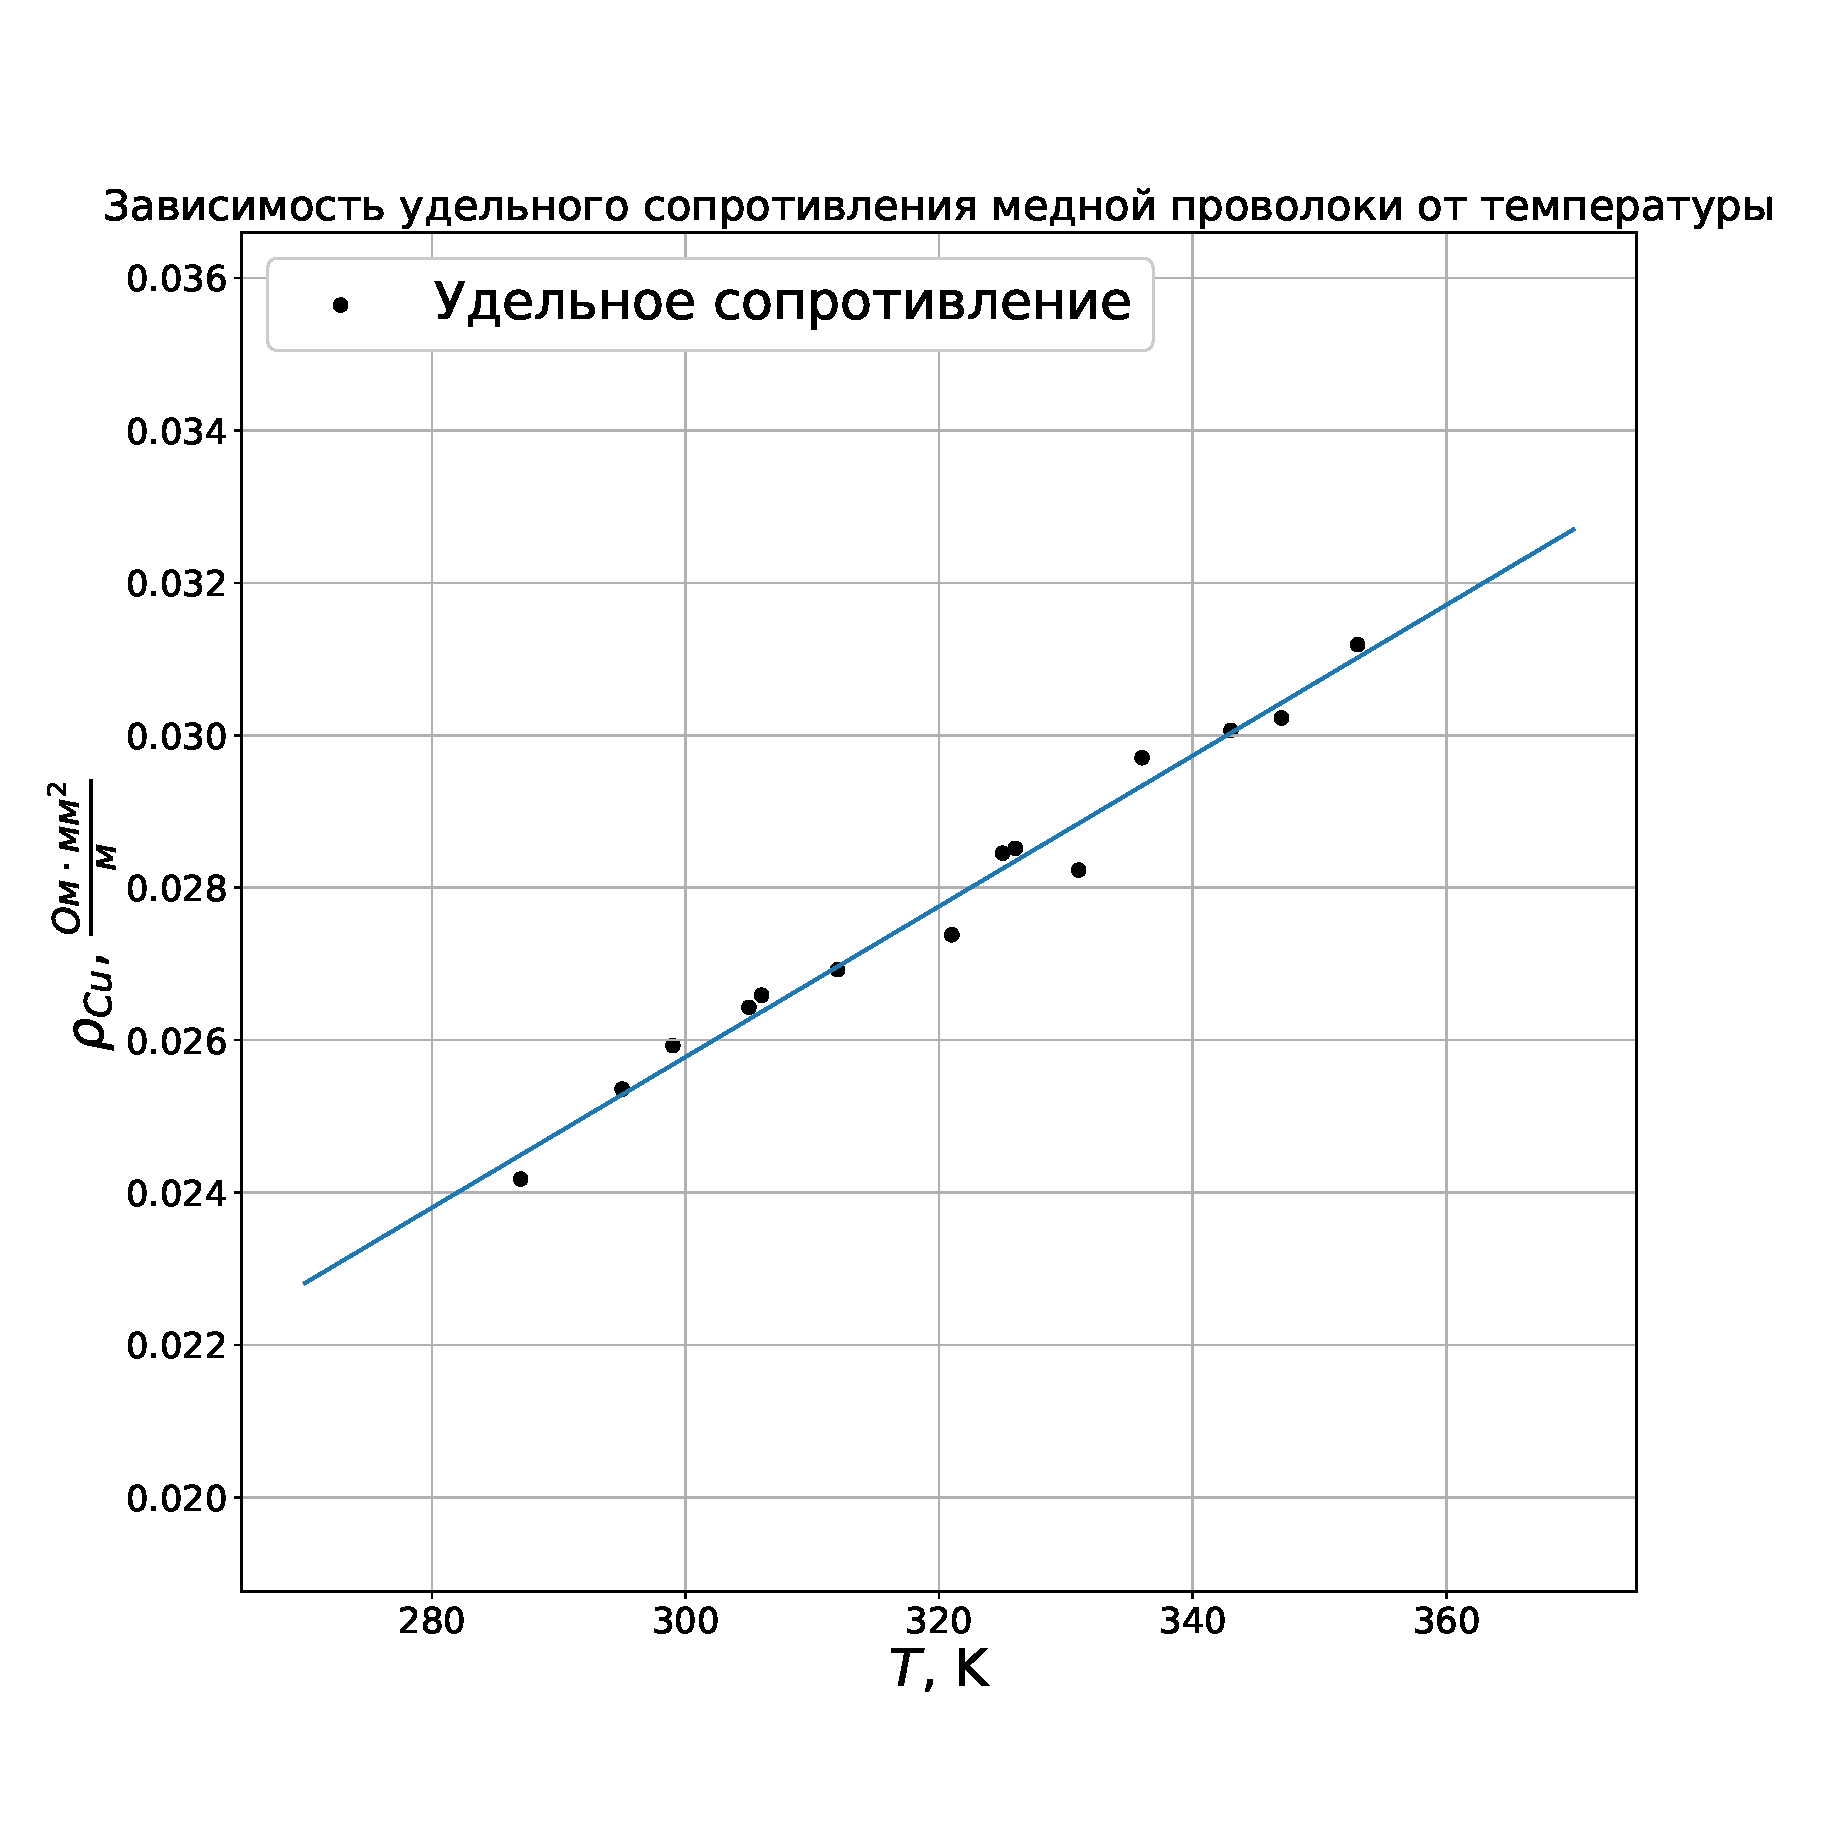
\includegraphics[width=.55\linewidth]{Lab3_2.eps}
			\caption{Получившийся коэффициент температурной зависимости сопротивления $\alpha \approx 3.9 \cdot 10^{-3}$ $\frac{1}{K}$ }
			\label{fig2}
		\end{figure}
	\end{center}
\end{frame}
\begin{frame}
	\frametitle{Ход работы}
	\framesubtitle{Измерение температурных коэффициентов}
	\begin{center}
		\begin{figure}[h!]
			\centering
			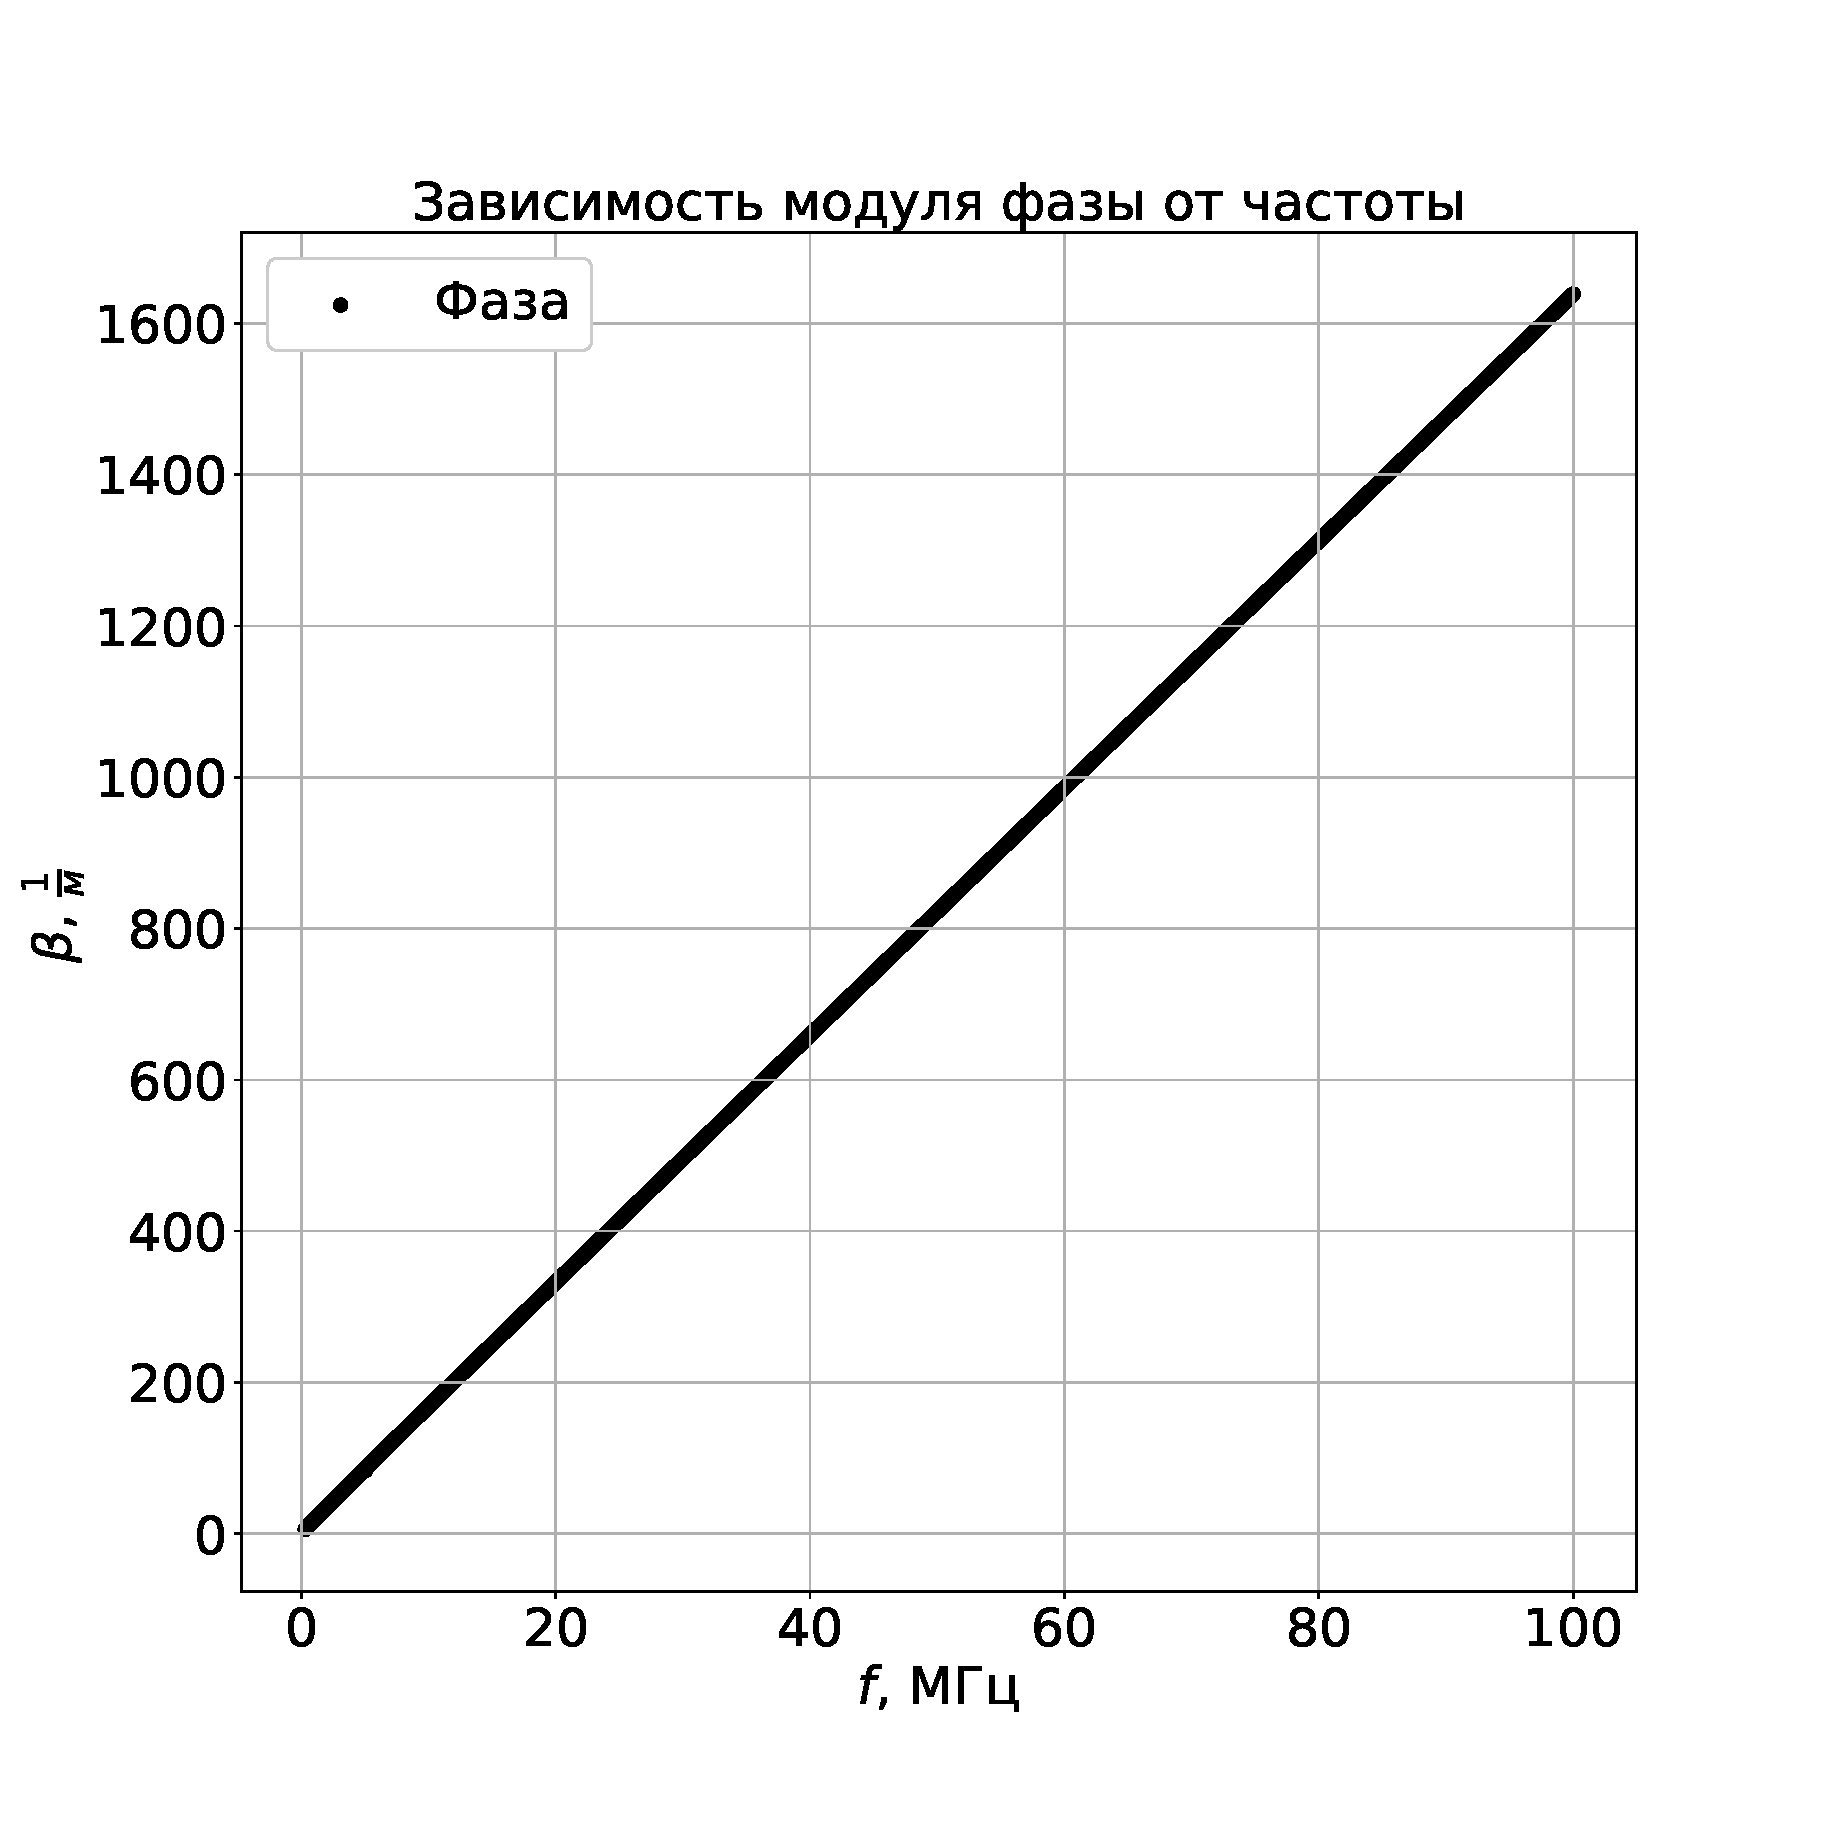
\includegraphics[width=.55\linewidth]{Lab3_3.eps}
			\caption{Получившийся коэффициент температурной зависимости сопротивления $\alpha \approx 127.6 \cdot 10^{-3}$ $\frac{1}{K}$}
			\label{fig3}
		\end{figure}
	\end{center}
\end{frame}
\begin{frame}
	\frametitle{Ход работы}
	\framesubtitle{Измерение температурных коэффициентов}
	\begin{center}
		\begin{figure}[h!]
			\centering
			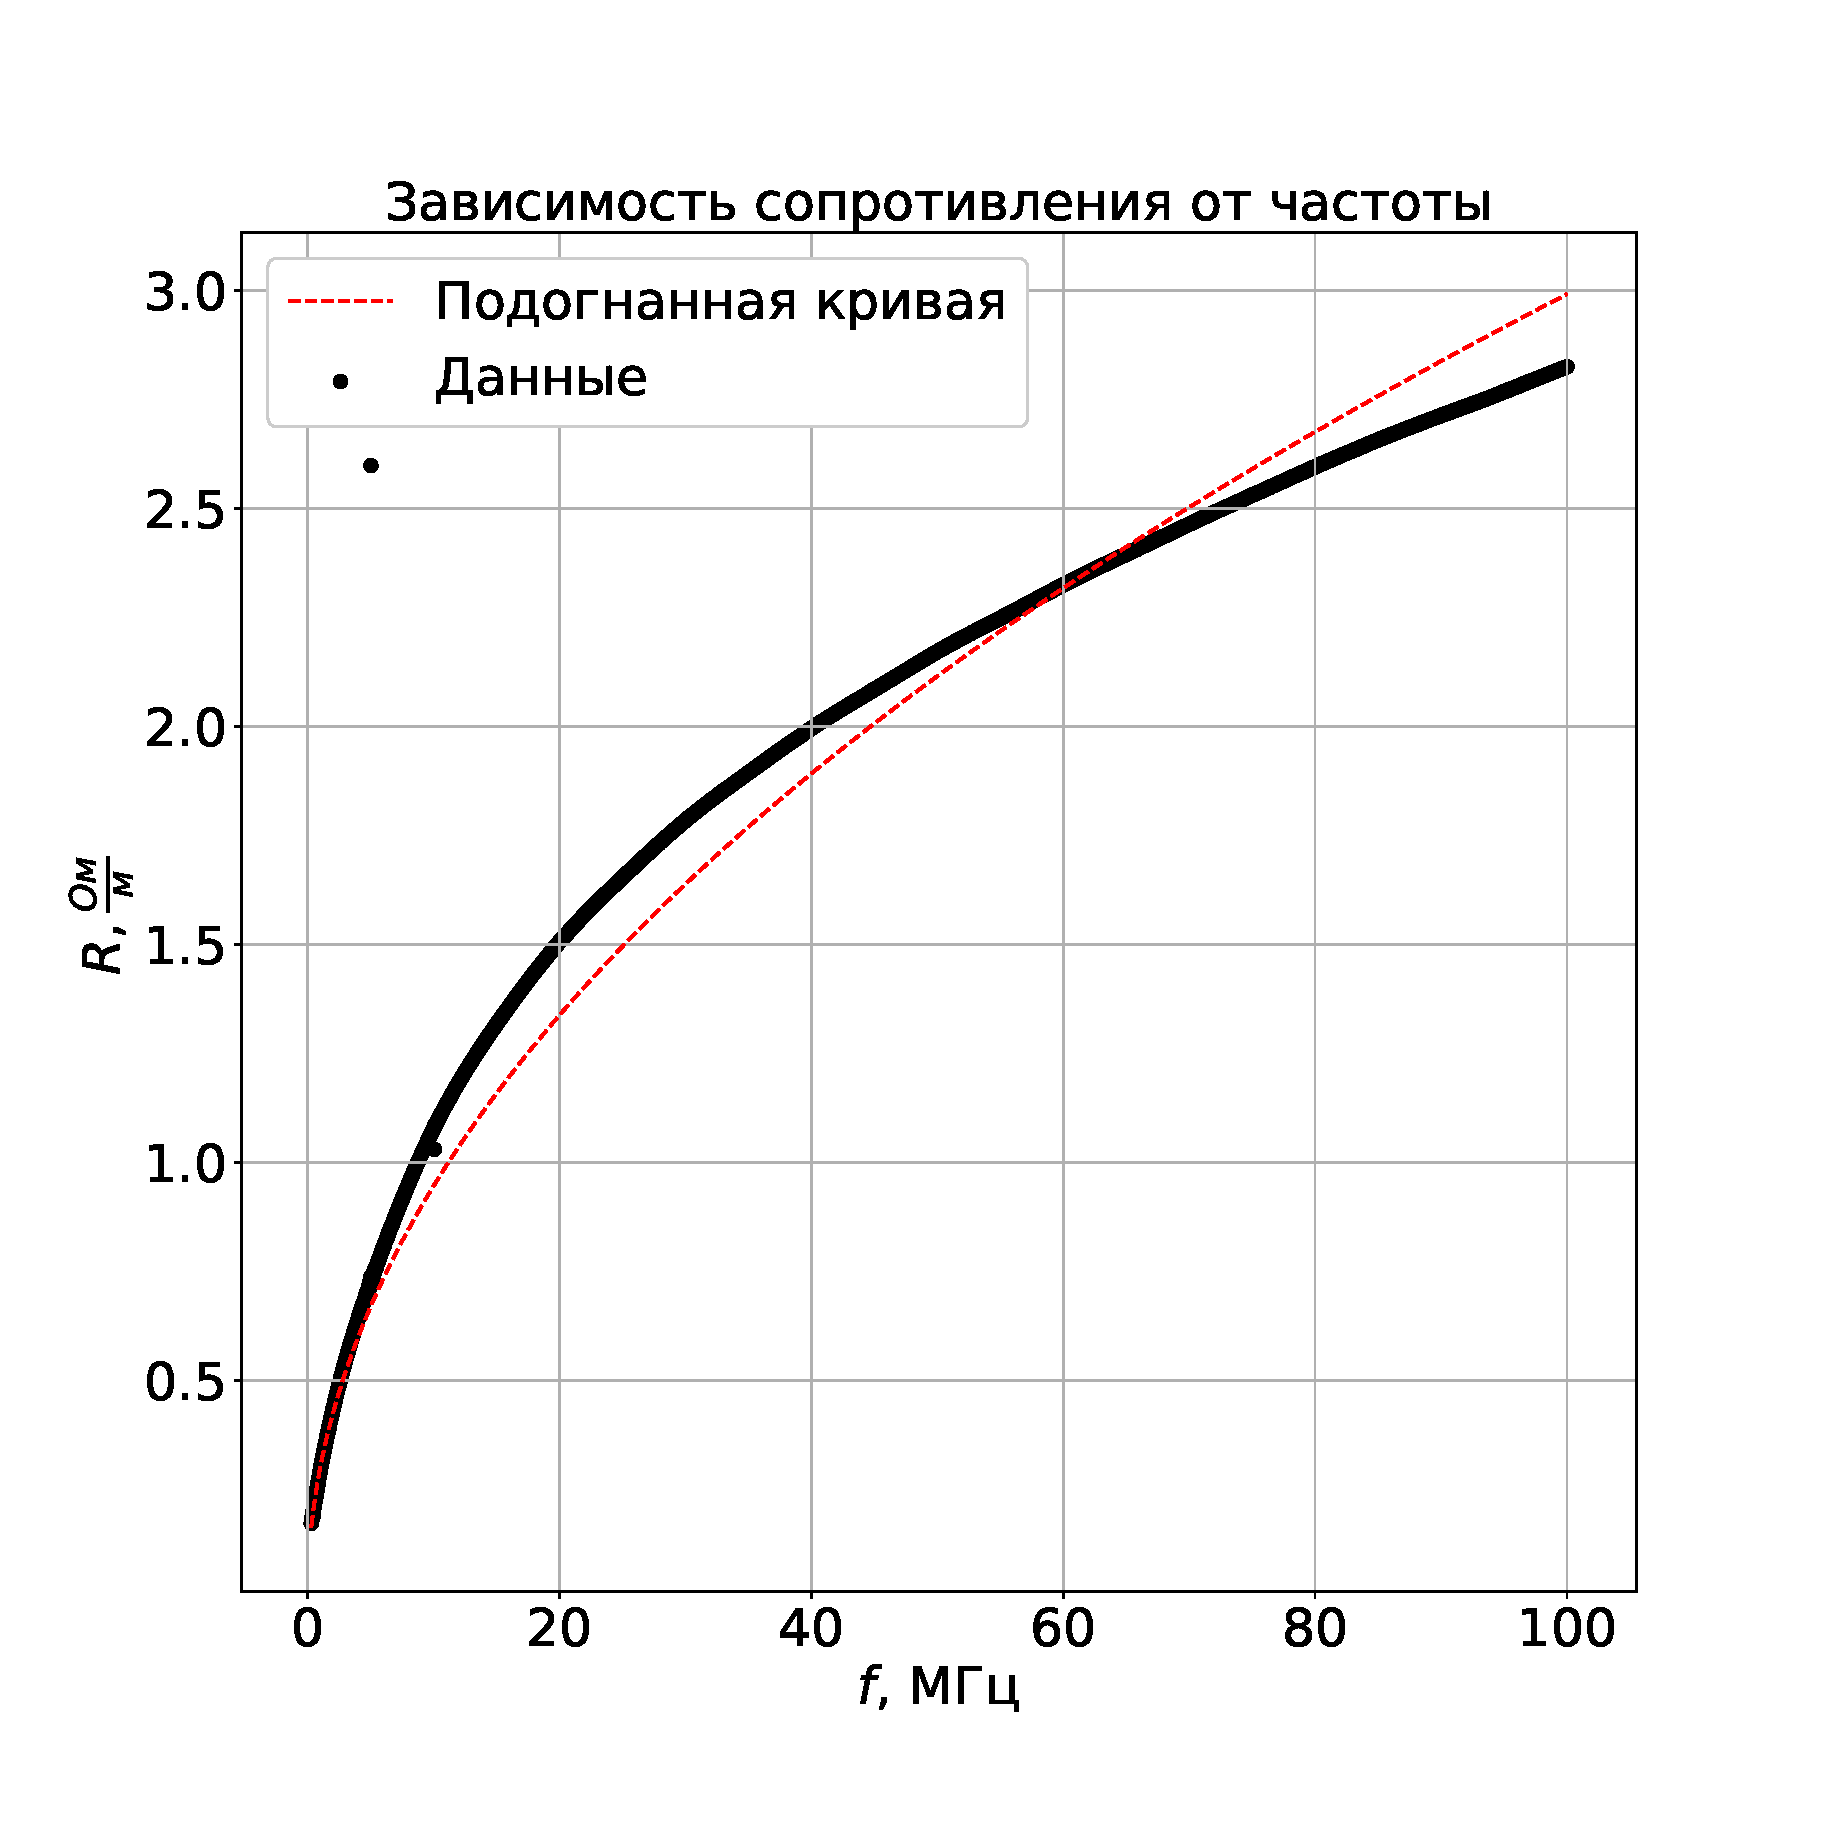
\includegraphics[width=.55\linewidth]{Lab3_4.eps}
			\caption{Получившийся коэффициент температурной зависимости сопротивления $\alpha \approx 2.3 \cdot 10^{-3}$ $\frac{1}{K}$}
			\label{fig4}
		\end{figure}				
	\end{center}
\end{frame}
\begin{frame}
	\frametitle{Ход работы}
	\framesubtitle{Измерение температурных коэффициентов}
	\begin{center}
		\begin{figure}[h!]
			\centering
			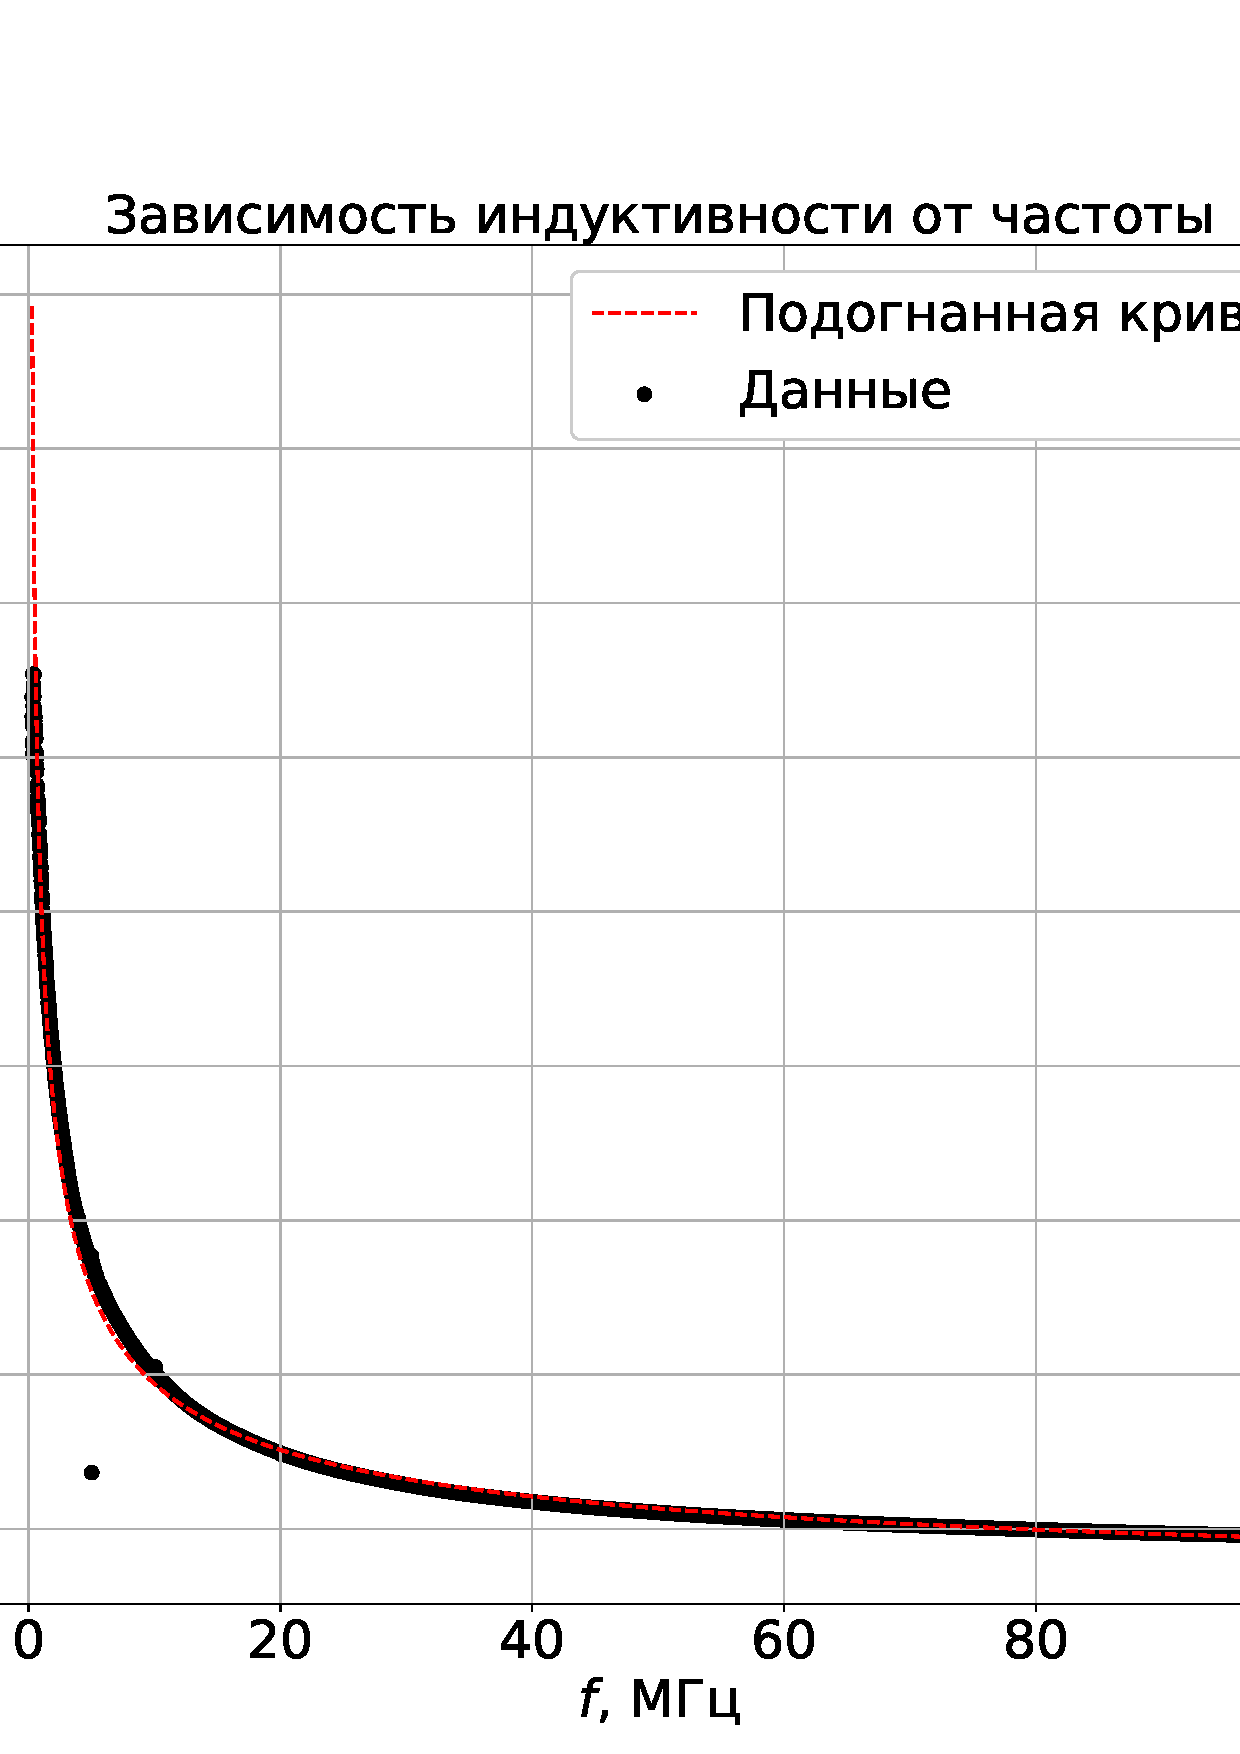
\includegraphics[width=.6\linewidth]{Lab3_5.png}
			\caption{Cхема подключения проволоки}
			\label{fig5}
		\end{figure}
	\end{center}
\end{frame}
\begin{frame}
	\frametitle{Ход работы}
	\framesubtitle{Измерение температурных коэффициентов}
	\begin{center}
			\begin{figure}[h!]
			\centering
			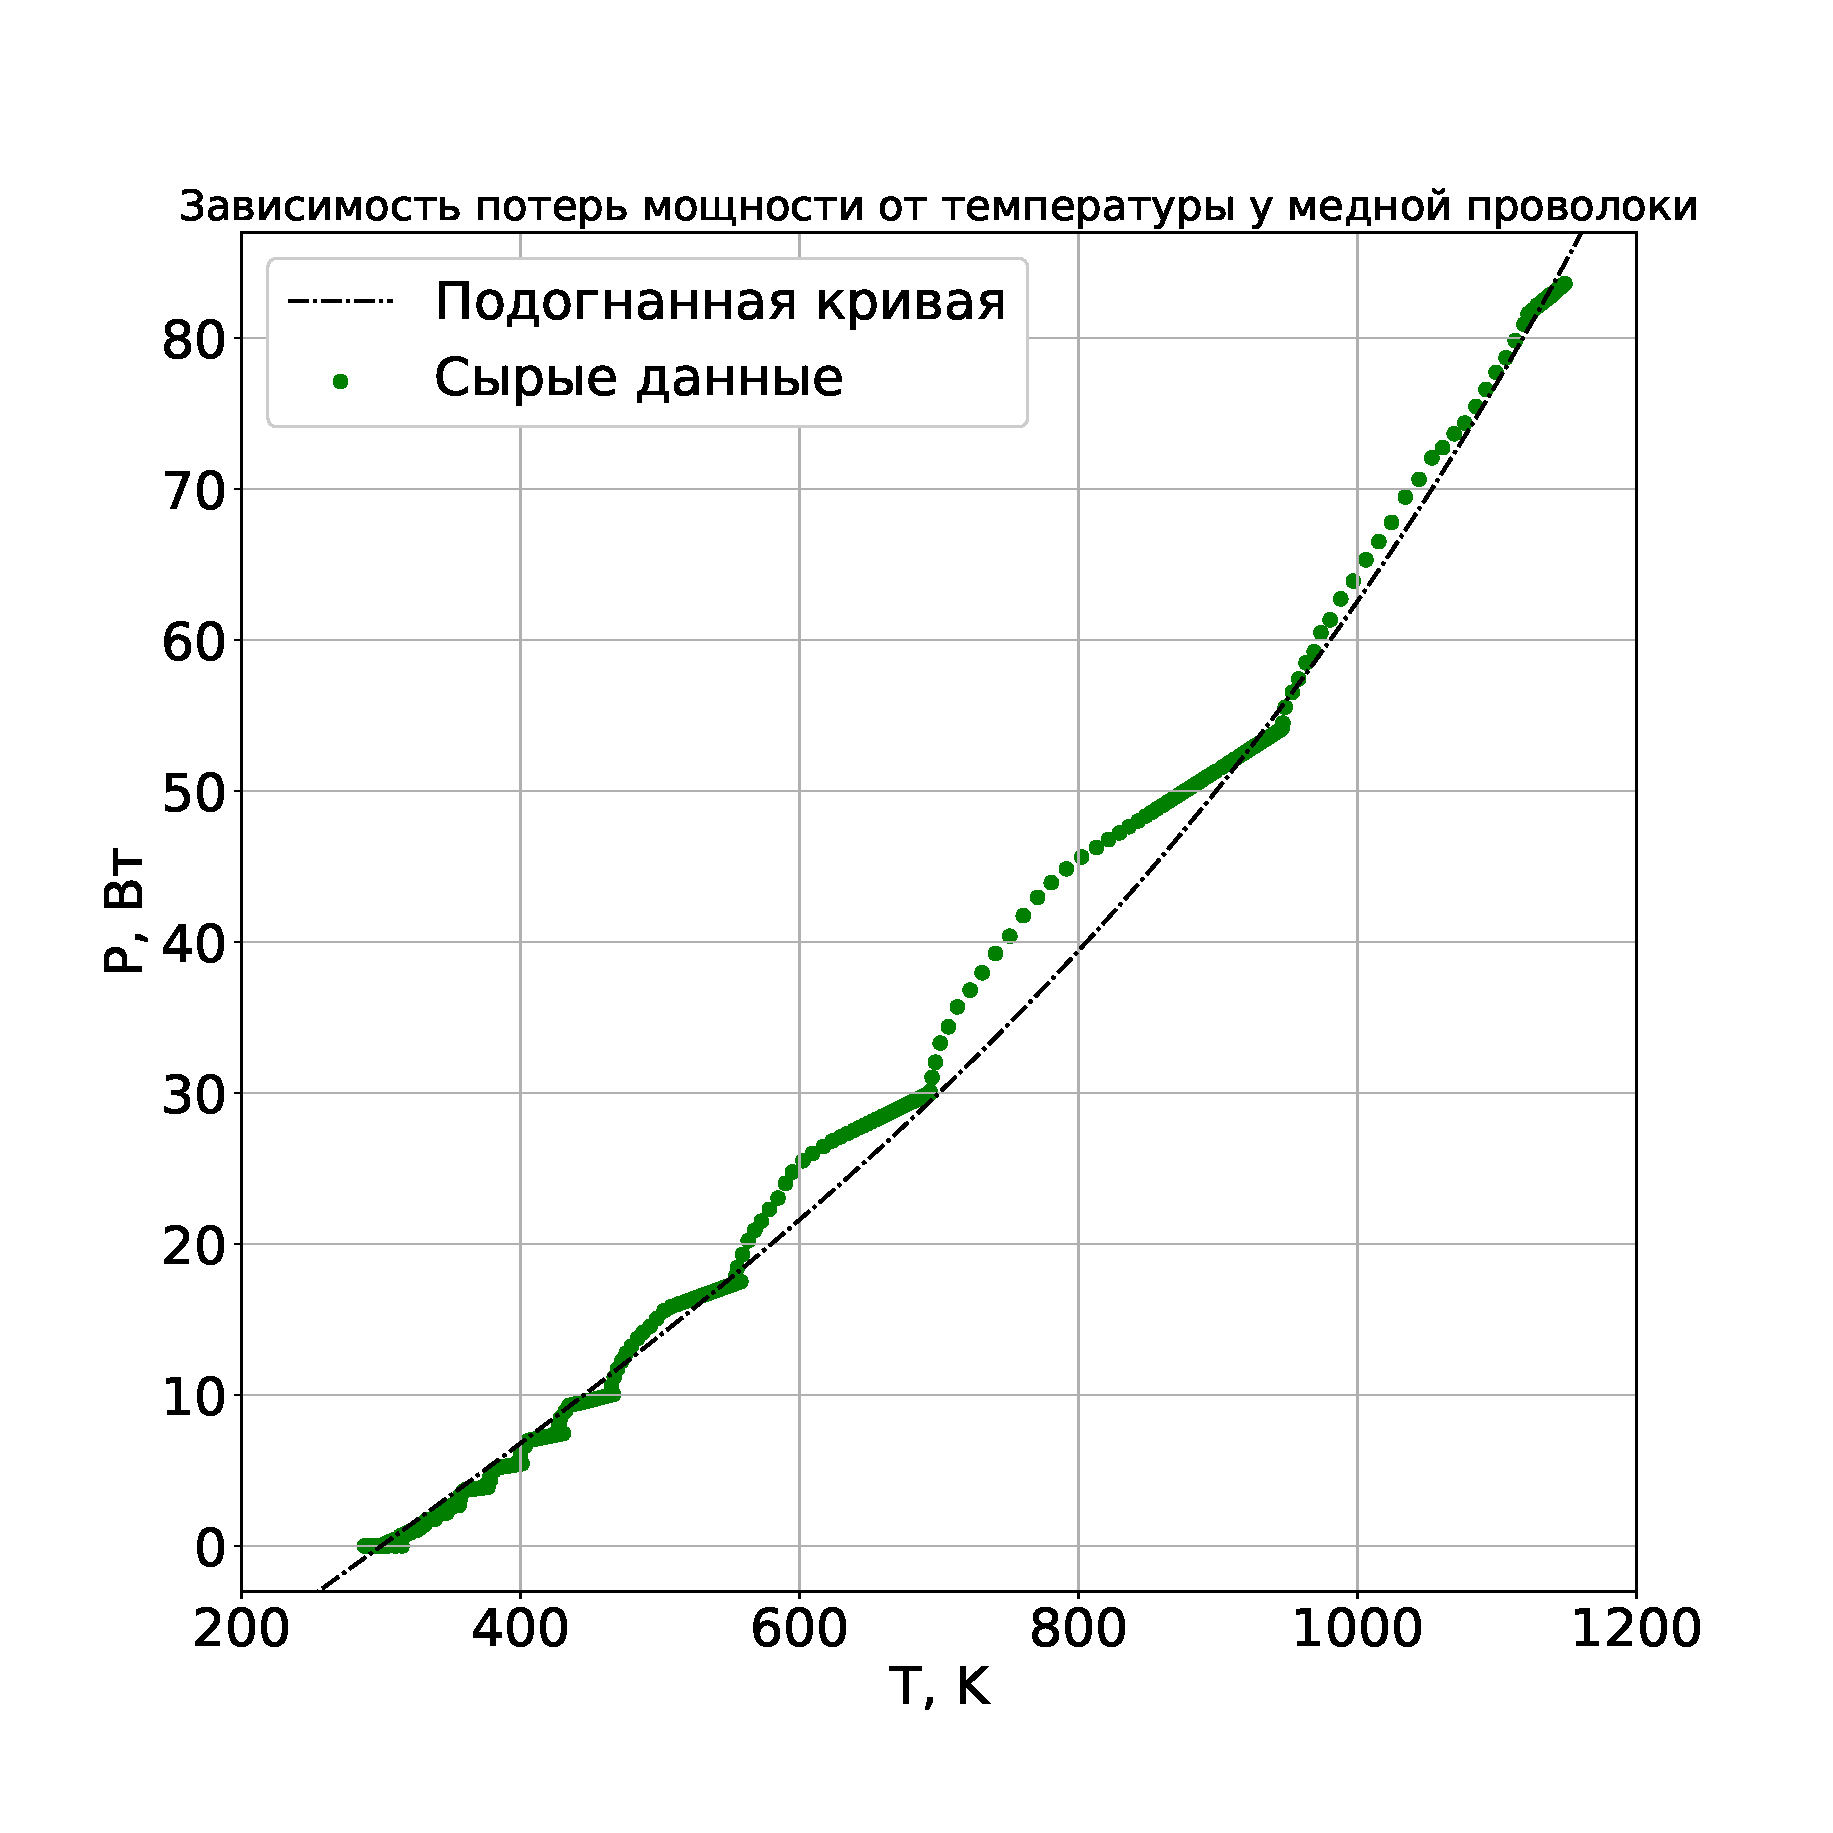
\includegraphics[width=.55\linewidth]{Lab3_6.eps}
			\caption{Коэффициенты $\beta \approx 52.9$, $\epsilon \approx 0.24$}
			\label{fig6}
		\end{figure}		
	\end{center}
\end{frame}
\begin{frame}
	\frametitle{Ход работы}
	\framesubtitle{Измерение температурных коэффициентов}
	\begin{center}
			\begin{figure}[h!]
			\centering
			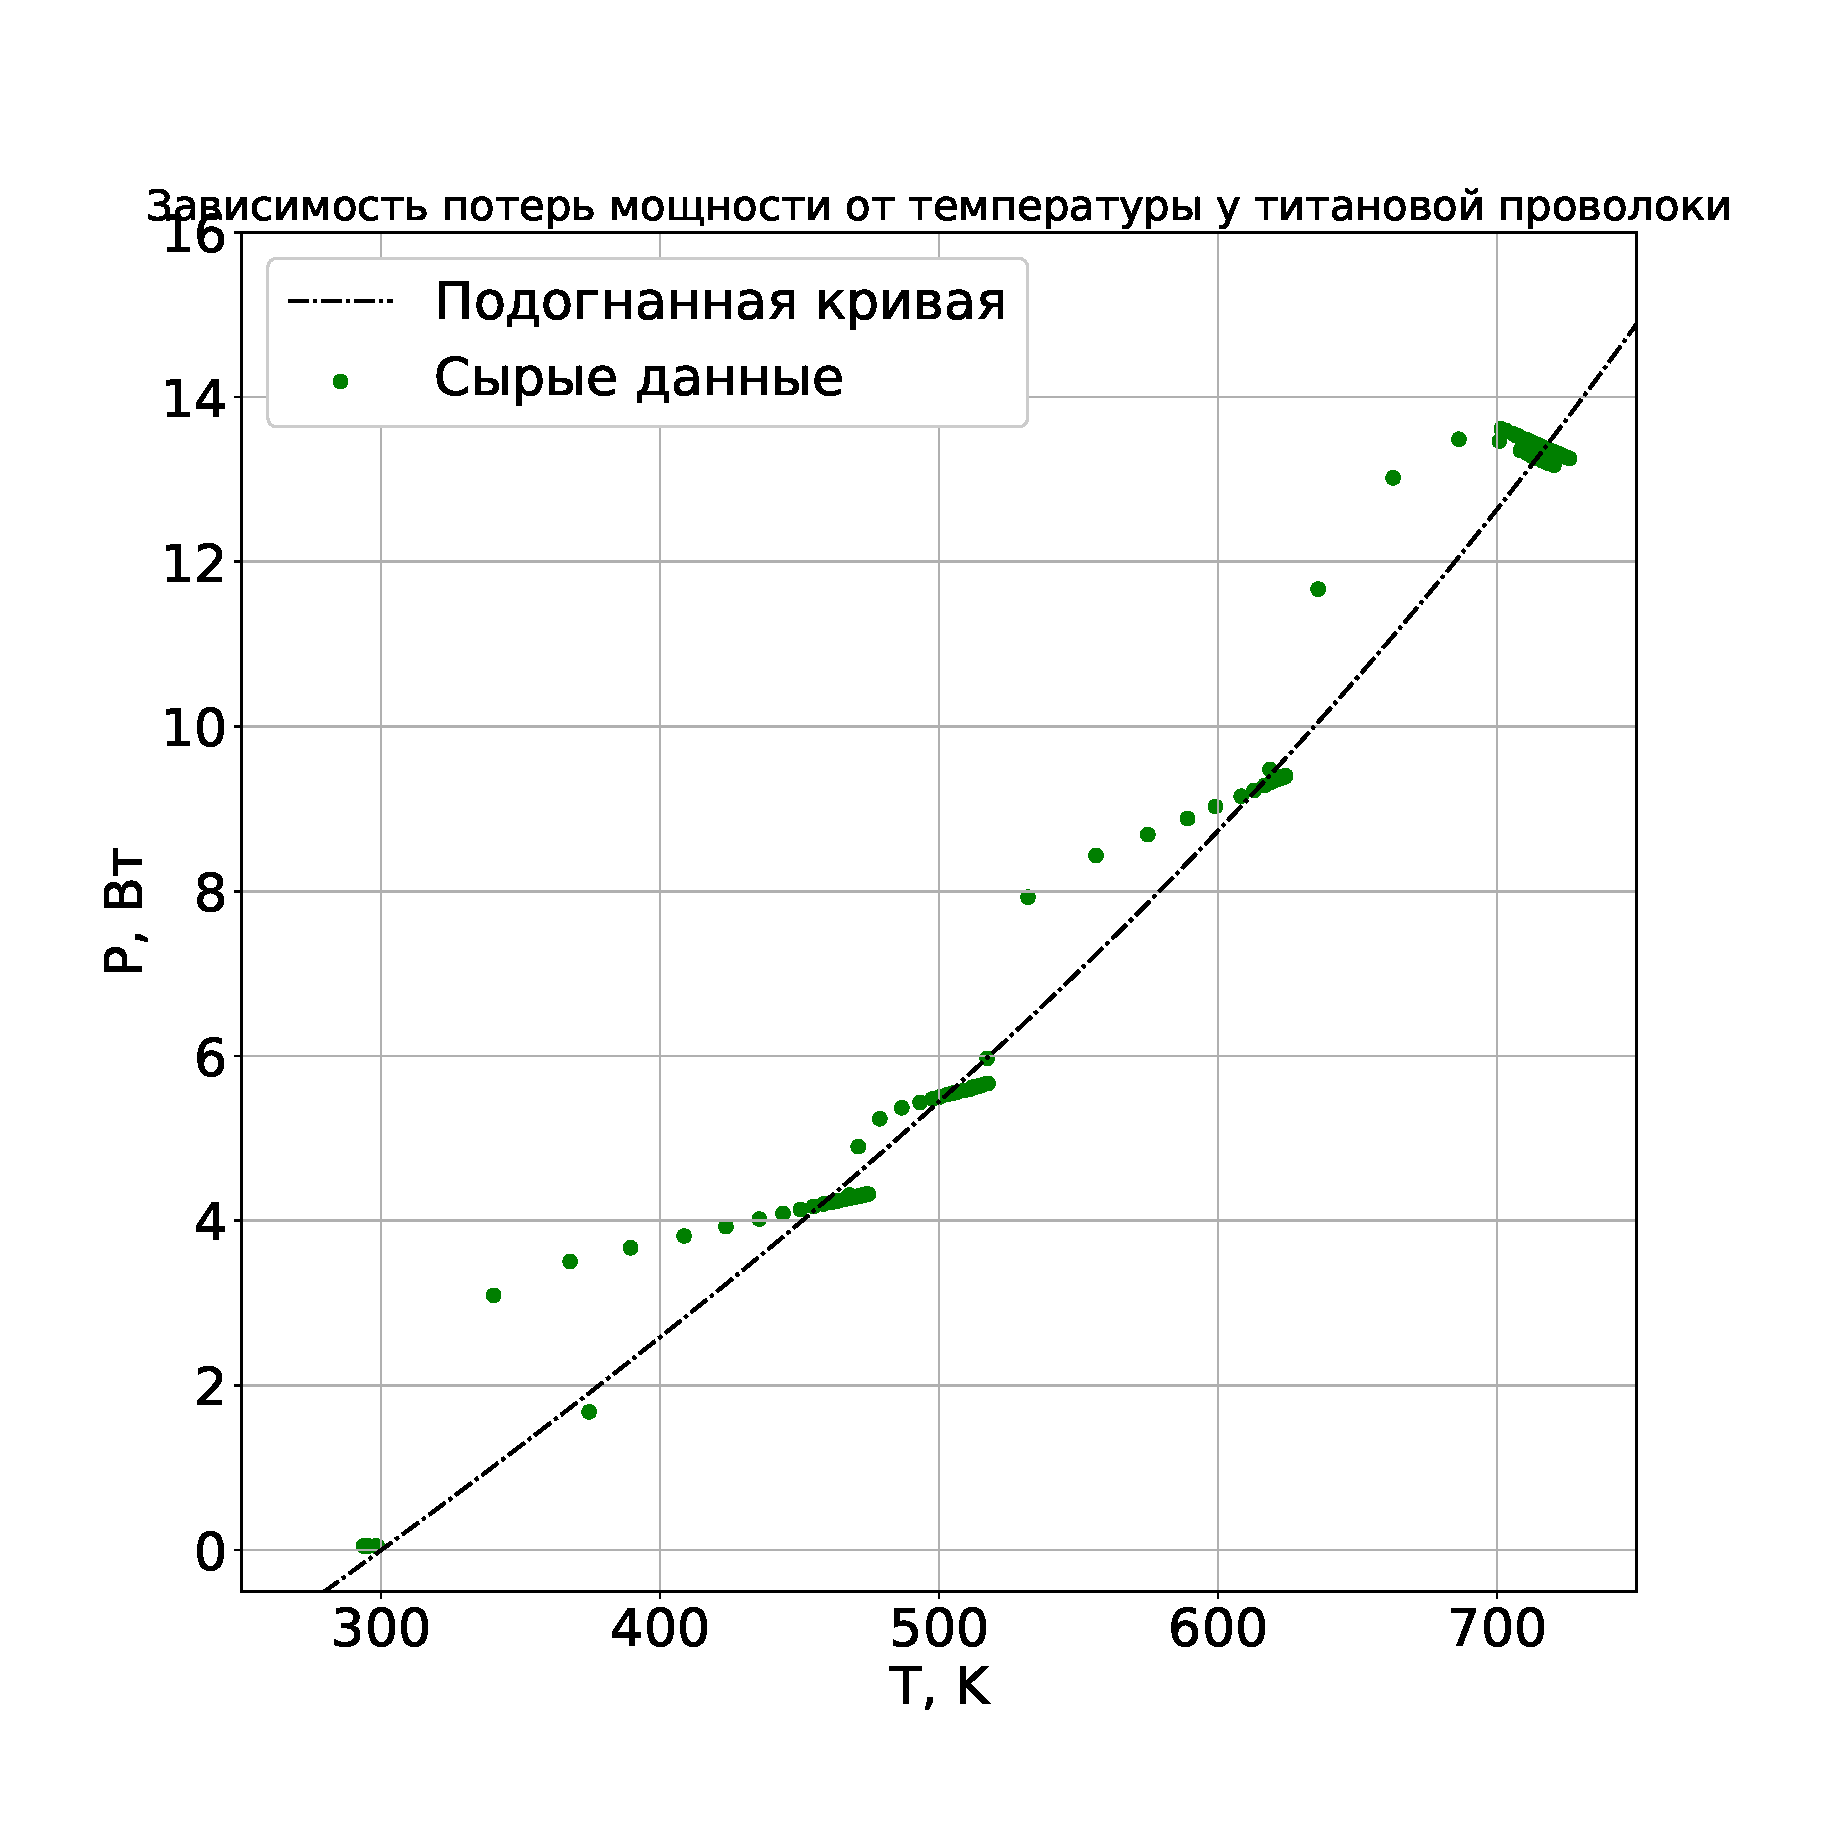
\includegraphics[width=.55\linewidth]{Lab3_7.eps}
			\caption{Коэффициенты $\beta \approx 27$, $\epsilon \approx 0.29$}
			\label{fig}
		\end{figure}		
	\end{center}
\end{frame}
\begin{frame}
	\frametitle{Ход работы}
	\framesubtitle{Измерение температурных коэффициентов}
	\begin{center}
			\begin{figure}[h!]
			\centering
			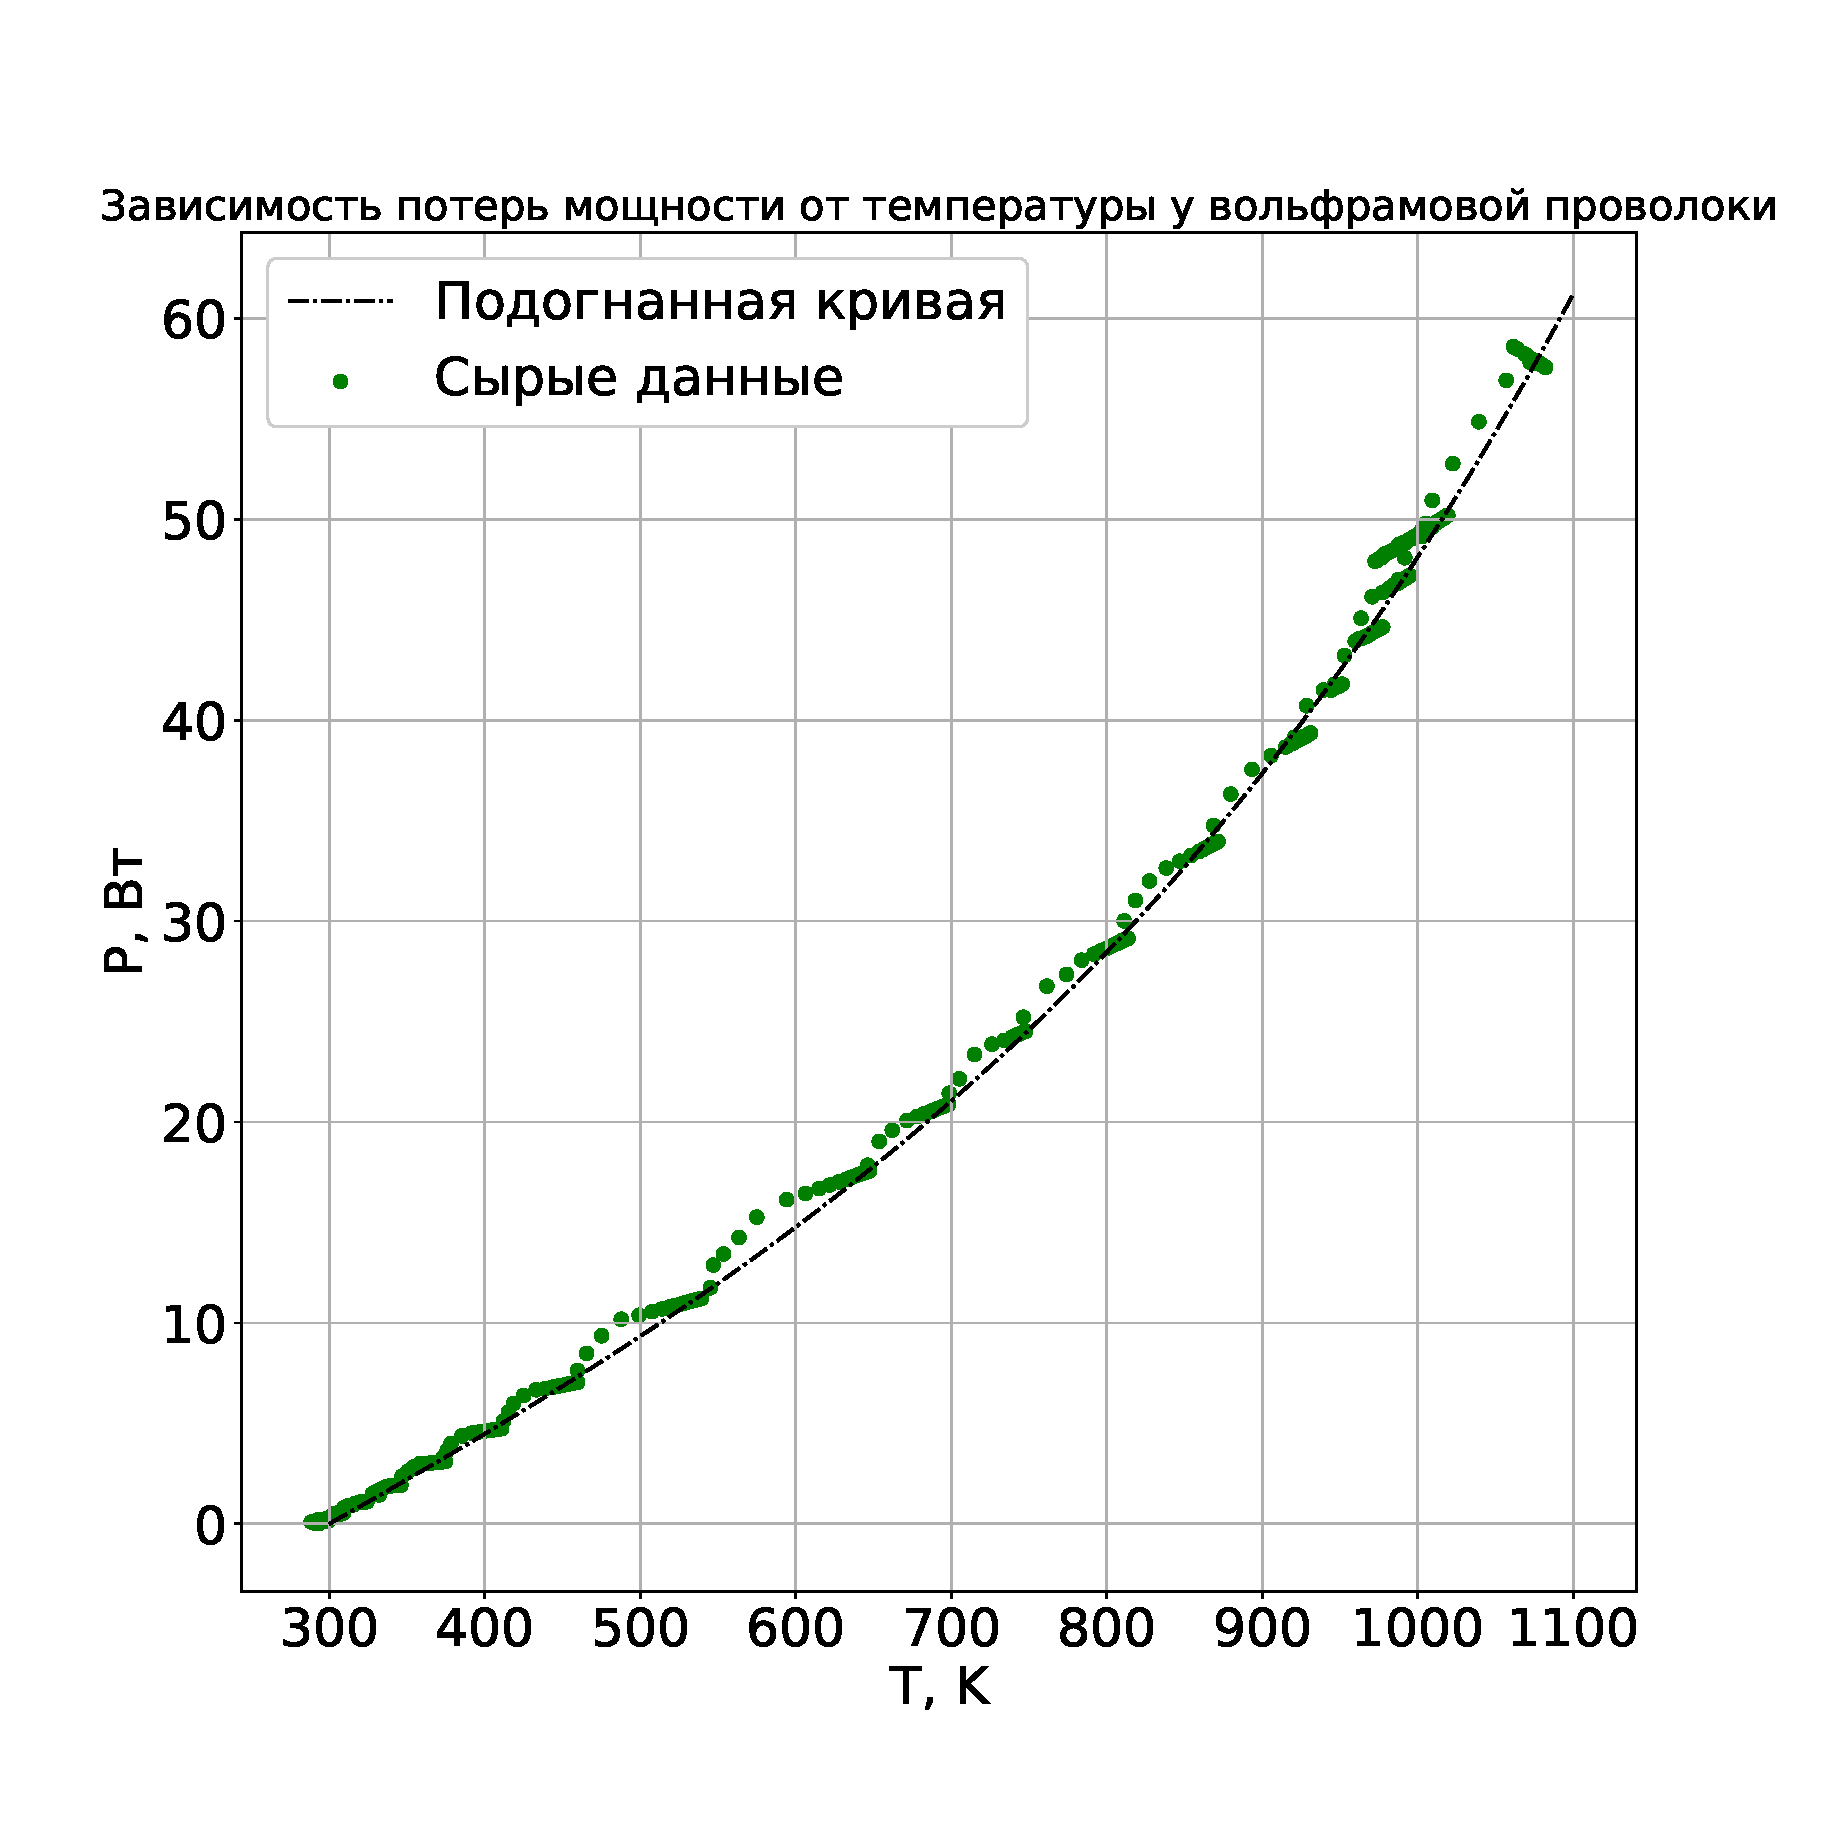
\includegraphics[width=.55\linewidth]{Lab3_8.eps}
			\caption{Коэффициенты $\beta \approx 47.1$, $\epsilon \approx 0.38$}
			\label{fig8}
		\end{figure}		
	\end{center}
\end{frame}
\begin{frame}
	\frametitle{Ход работы}
	\framesubtitle{Измерение температурных коэффициентов}
	\begin{center}
		Теплоемкость была посчитана в предположении, что энергия линейна по температуре и вся мощность уходит на нагрев образца (рассчеты произведены на температурах 200 - 400 K):
		\begin{equation}
			\begin{gathered}
				C_{Cu} = \frac{P \delta t}{m \delta T} \approx 435 \frac{\text{кДж}}{\text{кг} \cdot \text{г}} \\
				C_{Ti} = \frac{P \delta t}{m \delta T} \approx 620 \frac{\text{кДж}}{\text{кг} \cdot \text{г}} \\
				C_{W} = \frac{P \delta t}{m \delta T} \approx 170 \frac{\text{кДж}}{\text{кг} \cdot \text{г}}
			\end{gathered}
		\end{equation}			
	\end{center}
\end{frame}
\end{document}